\chapter{Introduction} % Main chapter title
\label{chp:introduction} 

%\todo{numbers!}

Modern online companies make broadly use of cloud computing infrastructures for 
carrying their business.
Among the cloud providers, the most popular and technologically advanced 
are Amazon Web Services (AWS), Microsoft Azure (Azure), and Google Cloud 
Platform (GCP)~\citep{flexera_report}.
To have a glance about the magnitude of their business, the second quarter of 
2020 showed a growth of $62$\% of Azure respect the same period in the 
previous year, with investments of $79.9$M USD, $78$M 
USD, and $76.7$M USD from Verizon, MSI Computer, and LG Electronics, 
respectively~\citep{azure_business}.
We can observer similar figures in Amazon AWS services, that declared $1$M of 
active users in 2020, with $18$M USD invested by Netflix in the same 
year~\citep{aws_business}.
Still in 2020, $786$ tech companies choose GCP for their 
businesses~\citep{google_business}.

The widespread of cloud computing technologies arose the attention of security
experts concerning the protections of third part 
infrastructures~\citep{ryan2011cloud,sun2014data}.
Check Point and McAffe surveyed the possible threats that could target
cloud services~\citep{checkpoint_cloud,mcaffee_cloud}.
Such problems reveal to be even more critical when considering that a huge part 
of could infrastructures (\ie the host machines) are out of the companies 
control.
In this scenario, leaving part of the control to the could provider means 
trusting that a list of issues are already addressed at vendor side (\eg Azure 
or AWS).
The source of risk are various, for instance, the cloud provider might suffer 
of insider threats, \eg a GCP's system admin could record the network traffic, 
access to the user's data, or tamper with the 
virtual machines (VM) themselves~\citep{insider_threat}.
In addition to these issues, recent works showed that two VMs, 
sharing the same host, can exchange information solely relying on the CPU 
cache~\citep{maurice2017hello}. This means that a VM can carry attacks 
toward other VMs on the same host.

Having a cloud infrastructure introduces security risks also for the final 
user. In fact, a remote client (\eg a smartphone) has no guarantees to 
communicate with the the correct software in the remote 
VM~\citep{beekman2016attestation}, \eg a malicious hypervisor may manipulate 
the physical pages and force a VM to load non-intended 
content~\citep{10.1145/3292006.3300022}.
Another source of insecurity comes from the stored data: passwords and critical 
information are saved in non-volatile devices (\ie hard-drives) that are under 
control of the cloud provider as well, thus inevitably leading to integrity and 
confidentiality issues.
In this scenario, classic cryptography solutions fail since the whole system 
might be compromised, \ie the cloud provider may control the cryptographic keys.
%
One could reduce the risk by adopting mitigation techniques, such as 
Trusted Platform Modules (TPM) to ensure software integrity at the boot phase 
\citep{tpm-isoosi}, sign strict contracts with the cloud providers to secure 
the underline system \citep{aws_dedicated_host}, or employing modern 
crptographic schemes to protect private data \citep{gentry2009fully}.
%
%such 
%as loading the intended software in a VM (\ie ), securing the underline system 
%(\ie 
%through strict contracts or dedicated hosts -- \cite{aws_dedicated_host}), and
%encrypting the private data (\ie using modern crptographic 
%schemes -- \cite{gentry2009fully}).
However, these solutions are rarely used in practice because either expensive 
or non scalalbe. The former requires dedicated hosts that are far more 
expensive than standard solutions, moreover TPMs are not common in the cloud 
offer. 
The latter, instead, involves heavy cryptographic schemes that slow down the 
computation, thus incompatible with fast response 
applications~\citep{10.1145/2046660.2046682}.
%
An addition source of threat is represented by classic exploitation techniques 
that may penetrate the system perimeter.
In this scenario, an adversary may target error-prone services exposed over the 
Internet, and take control of the
machines~\citep{van2012memory,10.1145/2810103.2813646}.
Finally infecting the system.

%\todo{possible solution: TEE. Give intuitive definition.}
For tackling the aforementioned challenges, a promises direction is 
represented by Trusted Execution Environments (TEE).
Intuitively, TEEs are sub-systems, whose functioning remembers virtual 
machines, that use string hardware checks to isolate their content against 
untrusted environments.
%\todo{Definition of TEE and usage. Properties, memory isolation, and remote 
%attestation.}
%\todo{History of TEEs, first definition, standard used, etc. During the 
%	description, stay "high level" and recall properties and differences. This 
%	should give a context.} 
The TEEs are controlled by the main CPU, that represents the primary source of 
trust, and enable a user to define \emph{trusted memory regions} in the main 
memory (RAM)~\citep{Sabt2015TrustedEE}.
Historically, the first formal definition of TEE has been proposed by OMTP, 
whose design was mainly focused on mobile platforms~\citep{omtp}.
OMTP defines a list of properties that a TEE should fulfill, among them, this 
thesis will trait the \emph{memory isolation} and the \emph{remote attestation}.
The main purpose of the \emph{memory isolation} is to shield code and data such 
that even a compromised machine cannot alter its integrity and confidentiality.
In particular, the \emph{memory isolation} must prevent tampering from any 
sources at any privilege level, \eg it must avoid writing and reading 
operations from the operating system, the SMM code~\citep{yao2009system}, and 
DMA transfers~\citep{coke1998implementing}.
The \emph{remote attestation}, instead, guarantees that a third party (\eg a 
smartphone) can verify the integrity of a remote memory region (\eg on a 
server).
This ensures that a client is communicating with the intended portion of code 
and machine (usually represented by the CPU).
The combination of \emph{memory isolation} and \emph{remote attestation} leads 
to a new range of properties in the cloud environments, \ie a company 
can use the \emph{memory isolation} to protect critical piece of 
software and data from insiders, a compromised host, or even other VMs sharing 
the same resources.
In addition, the \emph{remote attestation} allows the establishment of 
end-to-end secure channels without the support of the OS, thus avoiding the 
leak of cryptographic materials.
In addition, the TEEs can use attestation to seal data on non-volatile storage 
(\ie encrypt and decrypt) such that nobody but the original \emph{trusted 
region} can retrieve the content. 
TEEs are peculiar technologies that differ from previous solutions, such as TPM 
ones. Specifically, TMPs require an external hardware (\ie the TPM module), 
while TEEs are embedded in the main CPU.
Moreover, TPMs do not provide memory isolation, can only store limited 
cryptographic material (\eg keys), and expose a limited number functionalities 
already wired in the module by the vendor
(\eg random number generation or cryptographic primitives).
On the contrary, TEEs are meant to contain general purpose software that might 
interact with the peripherals.
In chapter~\ref{chp:background}, we detail the TEE background.

From the first OMTP definition, many vendors proposed their own TEE technology 
on the market.
In 2012, Intel proposed  Trusted Execution Technology 
(TXT) to measure the software integrity~\citep{greene2012intel}.
In 2014, ARM introduced the TrustZone technology in new lines of CPU and 
controllers~\citep{arm-trustzone}. 
%TrustZone devices can bootstrap two parallel OSs: one called \emph{enriched} 
%OS, that should handle all the normal operations; and a second one called 
%\emph{trusted} OS, with the duty to containing critical applications.
More recently, AMD proposed Secure Encrypted Virtualization 
(SEV) that shields whole VMs from their host~\citep{amdsev}, likewise,
Apple proposed a similar technology for their smartphones~\citep{apple-enclave}.
Among the various technologies, one particularly attracted the attention of the 
cloud market: Intel Software Guard eXtensions (SGX).
Intel SGX was announced in 2013~\citep{rozas2013intel} and is currently adopted 
by many cloud providers, such as Azure~\citep{azure}, 
GCP~\citep{challita2018precise}, IBM~\citep{IBM}, and 
Alibaba~\citep{alibabasgx}.
This technology provides either a strong \emph{memory isolation} and a reliable 
\emph{remote attestation} that stand at the backbone of many businesses, such 
as Signal~\citep{signal}.
Due to the important growth of SGX in the recent years, and considering its 
adoption in the cloud computing market, this thesis will consider SGX as main 
TEE technology.

\section{Software Guard eXtensions Overview}

The architecture of Intel Software Guard eXtensions (SGX) is synthesized in 
Figure~\ref{fig:sgx-architecture}.
The main concept of SGX are the \emph{enclaves}: memory regions in user-space 
physically isolated from the rest of the system.
SGX achieves \emph{memory isolation} due to a set of extra controls in the 
Memory Management Unit (MMU) and at micro-code level.
SGX considers the content of the \emph{enclaves} as trusted, and refers to them 
as \emph{trusted regions}, while the rest of the system is considered 
potentially malicious and is called \emph{untrusted region}.
The booting of an enclave is handled at kernel-space (\ie through a driver) in 
combination with extra CPU checks that ensure the correct \emph{enclave} 
loading.
Once an \emph{enclave} is bootstrapped, a remote entity can perform a 
\emph{remote attestation} (SGX RA) to verify the \emph{enclave} integrity.
The \emph{enclaves} live only in user-space and cannot directly 
interact with the kernel (\ie they cannot invoke \texttt{sycalls}).
The interaction between \emph{enclaves} and OS is handed by development 
frameworks that organize the enclave code in \emph{secure} and \emph{outside 
functions}.
The former are contained in the \emph{enclave} and handle critical pieces of 
code and data, while the latter are in the \emph{untrusted region} and interact 
with the system (\eg writing files, network communication).
We provide further details of the SGX internals in 
Section~\ref{sec:software-guard-extension}.

\begin{figure}[t]
	\centering
	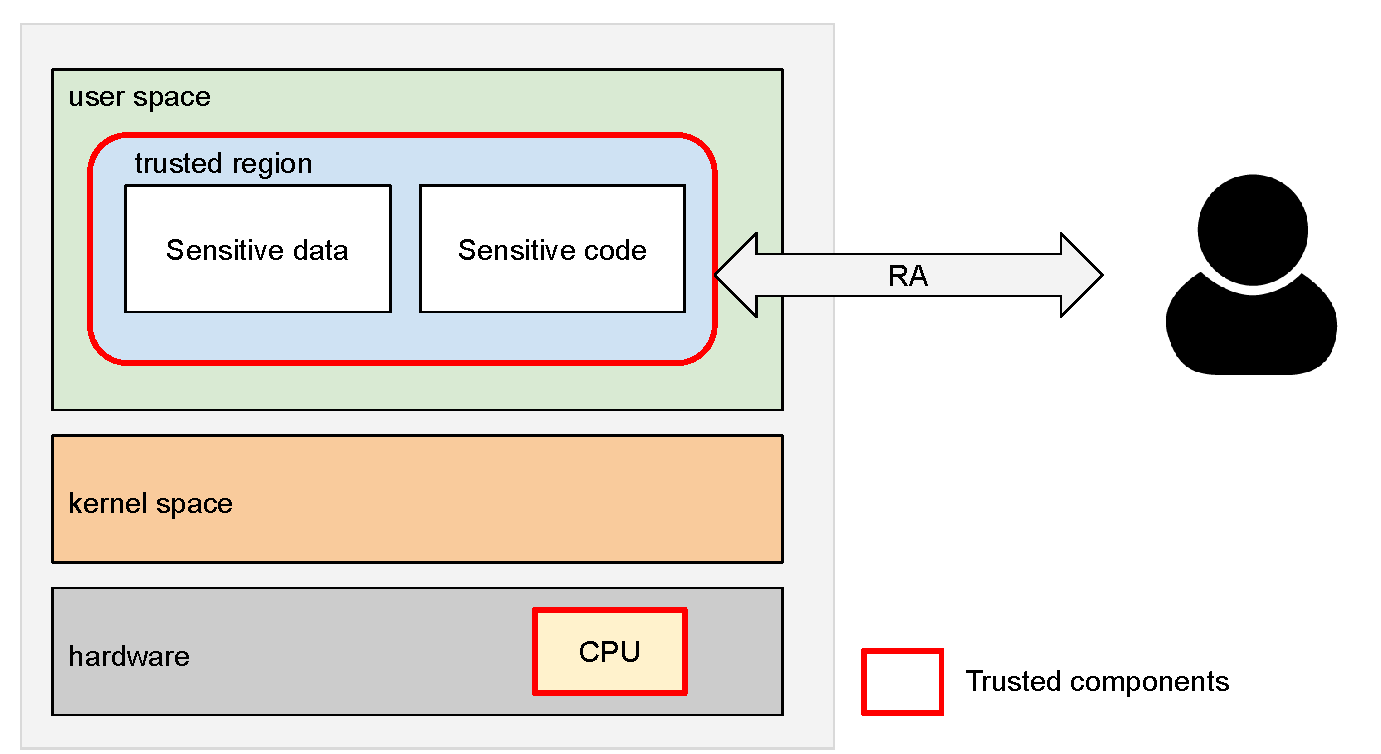
\includegraphics[width=0.7\textwidth]{fig_c1/sgx-architecture.pdf}
	\caption[SGX architecture.]{Simplified SGX architecture.}
	\label{fig:sgx-architecture}
\end{figure}

\section{Thesis Contribution}

%\textbf{MY THESIS OBJECTIVE:}
Regardless the security guarantees achieved by SGX, this technology still 
suffers of important limitations.
In this thesis, we argue we can improve the SGX security level (and in 
general of the TEE ones) through a shrewd software design without the need of 
changing the hardware specification.
Specifically, we identify four important areas to investigate, and for each of 
them we propose up to two contributions.
The thesis will describe five contributions in total that will 
address four aspect of SGX. The whole thesis contribution is summarized on 
Figure~\ref{fig:contribution}.

In the following, we summarize the four areas covered and the relative 
contributions. Finally, we elaborate each point in a dedicated section.

\begin{itemize}
	\item \textbf{Enclaves Scalability Limitations.} The whole memory dedicated 
	to SGX \emph{enclaves} is bounded to few mega bytes for machine. This 
	affects the amount of critical content that can be protected 
	contemporaneously.
	We study new software designs that stretch the SGX \emph{memory isolation} 
	over vaster memory areas while keeping a limited overhead 
	(Section~\ref{ssec:contribution1}).
	This is depicted by the symbol \circledr[1] in 
	Figure~\ref{fig:contribution}.
	
	\item \textbf{New Threats Led by Memory Isolation.} The \emph{memory 
	isolation} avoids an external observer to understand if an \emph{enclave} 
	contains benign or malicious software. Therefore, SGX could be used as a 
	nest for a new category of malware.
	We study to which extent an adversary can exploit SGX to introduce new 
	treats 	in a system (Section~\ref{ssec:contribution2}).
	This is depicted by the symbol \circledr[2] in 	
	Figure~\ref{fig:contribution}.
	
	\item \textbf{Remote Attestation Limitations.} The standard RA can only 
	guarantee that an \emph{enclave} has been loaded properly, but it does 
	not model runtime properties such as the execution-flow or the internal 
	state.
	We study how to extend RA schemes to fill this gap 	
	(Section~\ref{ssec:contribution3}).
	This is addressed with two contributions that are represented by the 
	symbols \circledr[3] and \circledr[4] in Figure~\ref{fig:contribution}.
	
	\item \textbf{Incident Response Limitations.} The introduction of 
	non-observable memory regions affects the incidents response in 
	case of intrusion. We thus study the limitation of current investigation 
	techniques in the context of SGX machines and propose new memory-forensic 
	methodologies to investigate the root-of-cause
	(Section~\ref{ssec:contribution4}).
	This is depicted by the symbol \circledr[5] in 
	Figure~\ref{fig:contribution}.
\end{itemize}

\begin{figure}[t]
	\centering
	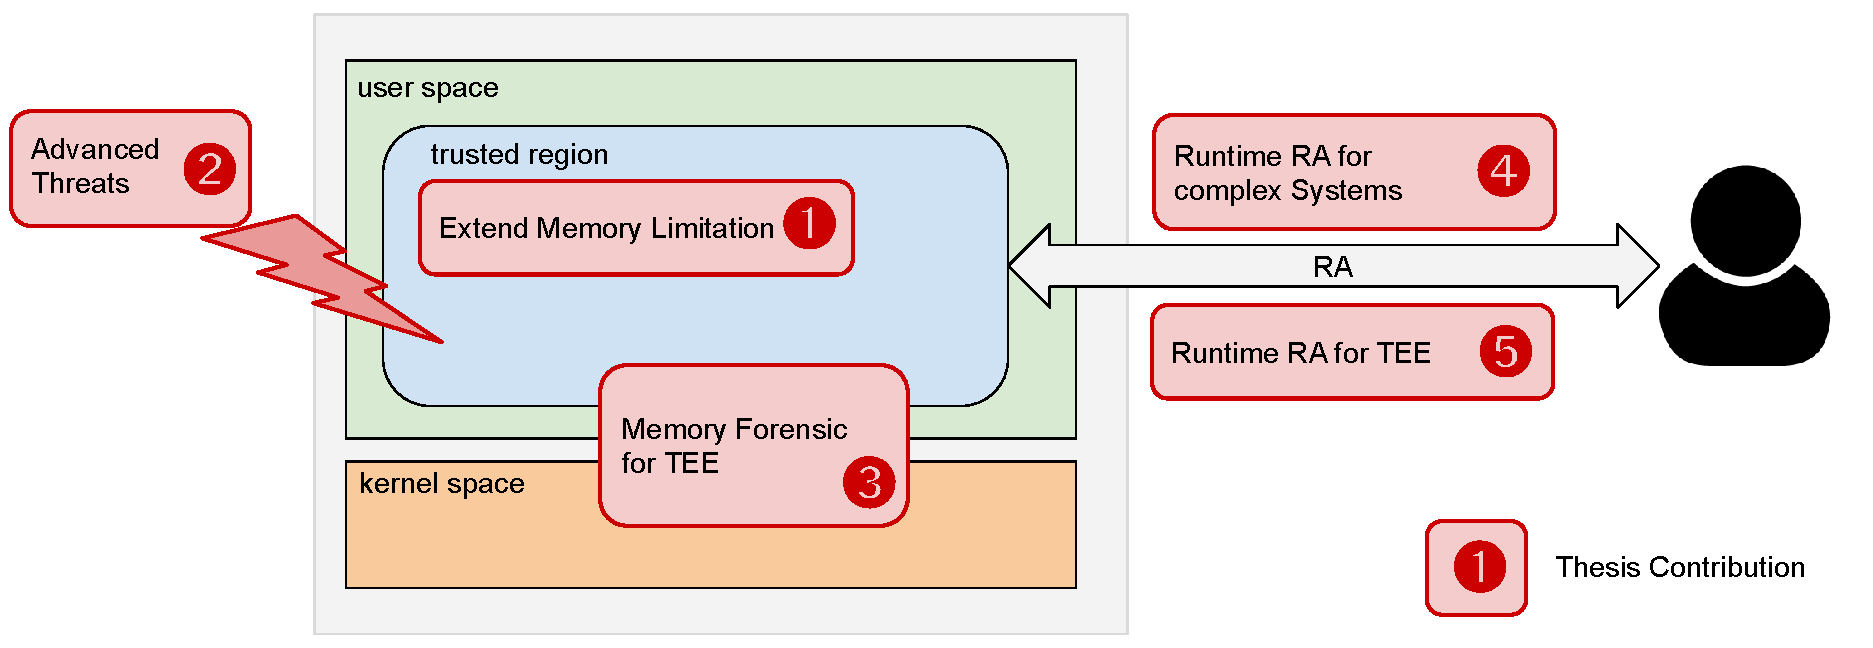
\includegraphics[width=\textwidth]{fig_c1/contribution.pdf}
	\caption[Thesis contribution.]{Thesis contribution.\todo{elaborate this 
	image and give a glance for each point.}}
	\label{fig:contribution}
\end{figure}

%\begin{figure}[t]
%	\centering
%	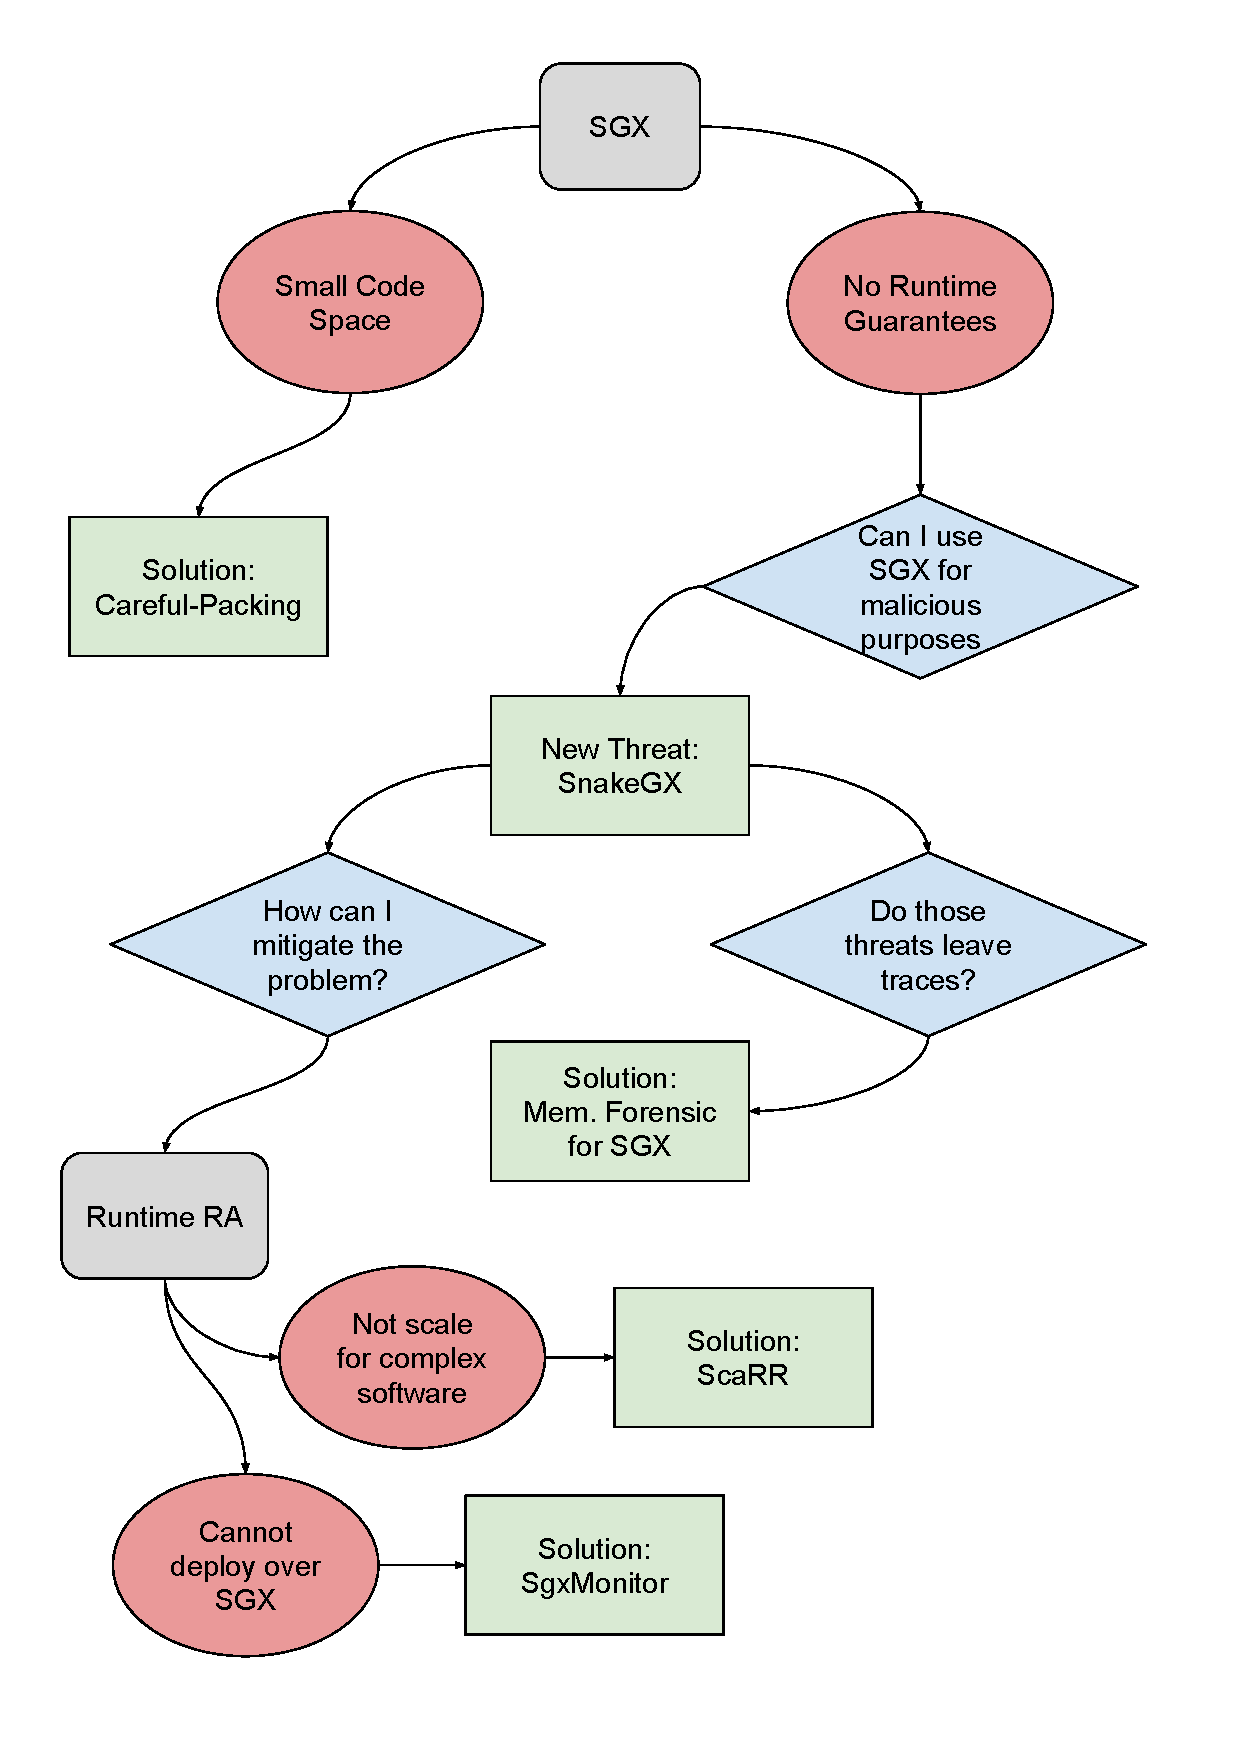
\includegraphics[width=\textwidth]{fig_c1/mind-map.pdf}
%	\caption[Mind-map.]{Mind-map (TO REMOVE LATER).}
%	\label{fig:mind-map}
%\end{figure}


\subsection{Enclaves Scalability Limitations}
\label{ssec:contribution1}

The \emph{memory isolation} of TEE modules is a strong protection against 
tampering attacks, which are commonly model as Man-At-The-End adversary (MATE).
In this scenario, the adversary may edit the binary code to alter the process 
logic~\citep{AKHUNZADA201544}, while the defender must guarantee that an 
adversary cannot change the software logic to some extent. 
TEE technologies, and in particular SGX, provide \emph{enclaves} 
that shield the software, thus avoiding MATE by design~\citep{costan2016intel}.
However, TEEs often have practical limitations, \eg software within an 
\emph{enclave} cannot directly interact with the hosting OS; and the enclave 
often has size limitations~\citep{baumann2015shielding}.
Previous works studied solutions that move part of the OS functionality inside 
a \emph{trusted 
region}~\citep{baumann2015shielding,arnautov2016scone,tsai2017graphene},
but they introduce further complexity for employing a secure interaction with 
the rest of the world (\eg networking, file system).
Other authors suggested protecting only portions of the 
code~\cite{schuster2015vc3,lind2017glamdring}.
However, these approaches do not address critical limitations such as the 
interaction with the underlying OS, or the limited amount of memory.
Limited memory makes it unsustainable to deploy all processes in dedicated 
trusted containers.
For instance, machines featured with SGX provide only a few hundred megabytes 
that must be shared among all the running \emph{enclaves}.
If we consider processes such as Skype or Firefox, which require around 
$100$MB each, we need multiple \emph{enclaves} for each process to protect.
Therefore, this approach does not scale for multiple parallel processes.
The introduction of SGX $2.0$ allows modifying the size of a single trusted 
container but it does not modify the maximum memory available for trusted 
containers.

As an alternative approach, researchers proposed anti-tampering techniques, 
that allow a software to inspect itself and check whether its code has been 
modified.
We refer to those techniques as \emph{self-checking}, which literally read the 
binary code of the protected software by using special functions called 
\emph{checkers}.
The checkers compute a digital fingerprint of the software bytecode and verify 
whether that fingerprint matches a pre-computed 
value~\citep{nagra2009surreptitious}. 
However, purely software-based anti-tampering techniques are not 
completely secure, since the defending mechanisms reside in an 
\emph{untrusted memory region} and a determined attacker can identify and 
disarm such defenses.
It is possible to harden anti-tampering techniques by using a combination of 
additional 
approaches that raise the bar for the attackers but that do not fundamentally 
address the 
problem~~\citep{horne2001dynamic,banescu2017tutorial,chen2016advanced,chang2001protecting,viticchie2016reactive}

Considering all the aforementioned problems, we propose to combine the 
anti-tampering techniques and the SGX isolation to extend code protection over 
\emph{untrusted region}.
Finally overcoming the intrinsic limitations of SGX.
We detail our contribution in Chapter~\ref{chp:static-protection}.

\subsection{New Threats Led by Memory Isolation}
\label{ssec:contribution2}

The SGX design, coupled with a full encryption of an enclave's content, provides
advanced protection mechanisms and a trusted communication channel between the
enclave and the host process (\ie the main application the enclave belongs to).
The success of SGX stems from its strict threat model, that considers the OS
malicious: one can thus tamper with applications, modify their
behavior, exfiltrate sensitive information, and so on~\citep{iagoattack}.
In this context, SGX disallows kernel- and user-space code to
manipulate enclave memory pages, thus guaranteeing integrity and
confidentiality in the presence of any Iago attacker.

The strong isolation introduced by SGX stimulated researchers and practitioners 
to develop new attacks 
vectors~\citep{foreshadow,Murdock2019plundervolt,203183,lee2017hacking}.
Among them, an interesting research line is to exploit memory-corruption 
errors inside the enclave code and run one-shot code-reuse attacks to steal 
enclave secrets (\eg cryptographic keys)~\citep{geometry2007}.
Recently, we observed many solutions that identify such flaws in 
enclaves~\citep{teerex,tale-two-worlds} and new code-reuse techniques 
tailored for SGX~\citep{lee2017hacking,biondo2018guard}.
First, \cite{lee2017hacking} discussed Dark-ROP that combines a colluded OS and 
oracles to identify gadgets for return-oriented programming 
(ROP)~\citep{geometry2007}.
The main limitation of this attack is the need of crashing the victim
enclave many times in order to craft the actual payload.
%An advanced technique was proposed by \cite{biondo2018guard} with Guard's 
%Dilemma that does not require the assistance of the OS 
%to perform the attack.
To cope with this issue, \cite{biondo2018guard} proposed Guard's 
Dilemma that uses particular gadgets already present in the Intel Software 
Development Kit (SDK) to build the payload without any enclave crashes.
Moreover, Dilemma requires only an unprivileged attacker to carry out a 
single one-shot attack and steal secrets from an enclave.


In this scenario, however, the previous authors did not consider an OS that may 
employ existing memory forensic techniques to identify the 
intrusions~\citep{stancill2013check,polychronakis2011rop,kittel2015counteracting,Graziano:2016:RFA:2897845.2897894}.
For instance, in case of external intrusion into a remote server running SGX 
enclaves, the adversary is also interested in reducing the amount of traces 
left; otherwise, analysts may detect the intrusion and act consequently.
This is even more critical in case the enclave secret changes and the adversary 
has to repeat the attack many times.

Considering all these challenges and the current state-of-the-art, we 
investigate if TEEs (and SGX in particular) can help adversaries carry more 
advanced threats by exploiting the TEE \emph{memory isolation}.
We detail our study in Chapter~\ref{chp:advanced-threats}.

\subsection{Remote Attestation Limitations}
\label{ssec:contribution3}

In standard Remote Attestation (RA) schemes, usually defined as static, the 
\emph{Prover} verification involves the integrity of specific hardware and 
software properties (\eg the \emph{Prover} has loaded the correct software).
On the market, there are already several available products implementing 
static RA, such as Software Guard Extensions (SGX)~\citep{costan2016intel} or 
Trusted Platform Module (TPM)~\citep{tomlinson2017introduction}.
However, these do not provide a defence against runtime attacks (\eg the 
control-flow ones) that aim to modify the program runtime behaviour. 
Therefore, to identify \emph{Prover} runtime modifications, researchers 
proposed runtime RA. Among the different solutions belonging to this category, 
there are also the control-flow attestation approaches, which
encode the information about the executed control-flow of a 
process~\citep{abera2016c,aberadiat}.

Studying the runtime RAs available in the literature, we identify two main 
limitations worthy of attention. 
First, we observed that current RAs are not suitable for complex systems, such 
as software running in cloud infrastructures.
Second, the current solutions cannot be employed in TEE technologies, such as 
SGX.
In the following, we explore these two limitations.

\paragraph{Runtime RA for Complex Systems.} 

In comparison to static RA, the runtime one is relatively new, and today there 
are no reliable products available on the market since researchers have mainly 
investigated runtime RA for embedded 
devices~\citep{abera2016c,zeitouni2017atrium,aberadiat,dessouky2017fat,Dessouky:2018:LLH:3240765.3240821}:
most of them encode the complete execution path of a \emph{Prover} in a single 
hash~\citep{abera2016c,zeitouni2017atrium,dessouky2017fat}; 
some~\citep{aberadiat} compress it in a simpler representation and rely on a 
policy-based verification schema; 
other ones~\citep{Dessouky:2018:LLH:3240765.3240821} adopt symbolic execution 
to verify the control-flow information continuously sent by the \emph{Prover}.

Even though the previous solutions result suitable for embedded devices, none 
of them can be applied to a complex system due to the following reasons: 
\begin{enumerate*}[label=(\roman*)]
	\item representing all the valid execution paths through hash values is 
	unfeasible (\eg the number of execution paths tends to grow exponentially 
	with the size of the program),
	\item the policy-based approaches might not cover all the possible attacks,
	\item symbolic execution slows down the verification phase.
\end{enumerate*}
Therefore, we study a new model that tackle these challenges and can represent 
complex software in limited space, thus can be adopted in cloud 
infrastructures. 
We describe our study in Chapter~\ref{chp:runtime-protection-untrusted}.


\paragraph{Runtime RA for SGX.}

SGX guarantees a \emph{trusted region} is properly loaded in memory, while 
static RA allows a remote entity to verify the correct enclave initialization.
As such, the SGX alone has no mechanisms to guarantee the correct runtime 
execution of enclaves, which remain vulnerable against
attacks aimed at causing deviations from enclaves' expected legitimate
behaviors~\citep{tale-two-worlds,251582,biondo2018guard,lee2017hacking,snakegx}.

The SGX \emph{memory isolation} exacerbates runtime attacks that target 
software loaded in enclaves, since there is no mechanism to 
monitor their executions and set legitimate and anomalous ones apart.
Although one can equip the enclaves with mechanisms tailored at counteracting 
specific threats, research has shown such solutions are brittle and cover a 
limited threat model, mostly focusing on code-reuse attacks, while neglecting 
vectors that induce deviation from normal
behaviors~\citep{tale-two-worlds,251582,biondo2018guard,lee2017hacking}.
Moreover, current runtime remote attestations focus on
stateless properties, \ie they only model independent executions.  On
the contrary, TEEs are stateful objects modeled as finite states
machines (FSM), as described by \cite{costan2016intel}.
Therefore, they require more complex representations.

After observing all these limitations, we study a runtime RA that can be
employed in SGX enclaves. We describe our study in 
Chapter~\ref{chp:runtime-protection-trusted}.

\subsection{Incident Response Limitations}
\label{ssec:contribution4}

Then addressed in Chapter~\ref{chp:forensic}.

